\section{Introduction}
In 2005 Grigory Mikhailkin showed that the number of degree $d$ plane tropical curves passing through $3d-1$ points, $N^{\text{trop}}_{d}$ is same as the number of plane rational curves $N_{d}$.
This result brought tropical geometry into the eyes of the wider mathematical community, and also gave rise to a new array of research problems.
In this chapter we are going to look at Gathmann and Markwig's work which proved Kontsevich's curve counting formula for tropical curves without making use of Mikhailkin's correspondence result.

\subsection{Overview of Proof Idea}
Before we show how to proceed with this count of tropical curves, it's instructive to look at the proof from the previous chapter for general ideas.
The proof in for rational plane curves in chapter 2 followed the following steps:
\begin{enumerate}
    \item For degree $d$ curves, we considered the moduli space $\overline{\mathcal{M}}_{0,3d}(\mathbb{P}^{2},d)$.
    \item The subvariety $Y \subset \overline{\mathcal{M}}_{0,d}(\mathbb{P}^{2},d)$ defined by:
        \[
            Y:= \nu_{1}^{-1}(L_{1}) \cap \nu_{2}^{-1}(L_{2}) \cap \nu_{3}^{-1}(Q_{1}) \cap \dots \cap \nu_{3d}^{-1}(Q_{3d-2}),
        \]
        corresponds to the set of degree $d$ curves passing through the lines $L_{1}$ and $L_{2}$ and points $Q_{i}$.
    \item For the forgetful map, $\eta: \overline{\mathcal{M}}_{0,3d}(\mathbb{P}^{2},d)\to \overline{\mathcal{M}}_{0,4}$, look at the inverse image divisors of $D(m_{1}, m_{2}|p_{1}, p_{2})$ and $D(m_{1}, p_{1}|p_{2}, m_{2})$.
        Since these divisors are linearly equivalent we get the relation, 
        \[
            Y \cap D(m_{1}, m_{2} | p_{1}, p_{2}) \equiv Y \cap D(m_{1}, p_{1} | m_{2}, p_{2}).
        \]
    \item Equating the degrees of the divisors on the two sides of the above relation we obtain Kontsevich's formula.
\end{enumerate}

Ideally we would like to repeat these same steps in the tropical setting to obtain the curve counting formula, but we lack the tools to do so.
The moduli spaces of tropical curves aren't as well behaved as moduli spaces of rational plane curves.
In fact, the moduli space of tropical curves isn't even a tropical variety.
Further, we don't have a rich theory of divisors to rely upon for tropical varieties. 
But we do have enough tools in the tropical world to sketch out a proof of the curve counting formula in the spirit of Chapter 2.
\par To define an equivalent of the space of stable maps we need some sort of parametrisation of tropical curves. 
Since plane tropical curves resemble graphs we parametrise them with a set of graphs.
We then define moduli spaces of these graphs, and and their parametrisations - taking inspiration from $\overline{\mathcal{M}}_{0,n}$ and $\overline{\mathcal{M}}_{0,n}(\mathbb{P}^{r},d)$ respectively.
Although the modulis spaces we construct don't have nice properties like a theory of divisors, we can still define evalutation and forgetful maps like earlier.
The existence of these maps allows us to, in essence, mirror the proof from Chapter 2 via the following ideas.
\begin{enumerate}
    \item We first consider the Moduli space of parametrisations of plane tropical curves.
    \item Let $\overline{M}_{0,4}^{\text{trop}}$ denote the space of the graphs which parametrise tropical curves with $4$ marked points, with $\eta$ being the forgetful map to this moduli space.
    \item To deal with the lack of divisors, we combine steps $3$ and $4$ from above to define a map,
        \begin{align*}
            \pi = \text{ev}_{1}^{1} \times \text{ev}_{2}^{2} \times \text{ev}_{2} \times \dots \times \text{ev}_{n} \times \eta,
        \end{align*}
        considering the intersections of $Y$ with element of $\eta^{-1}\overline{\mathcal{M}}_{0,4}$ directly insted.
    \item We show that the degree of this map counts curves in a similar manner as those of intersection divisors, and by using the fact that its degree is contsant we derive Kontsecivh's formula.
\end{enumerate}

\section{The Prerequisites}
The enumerative problem we are going to tackle just considers tropical curves in $\mathbb{R}^{2}$.
As we saw in Chapter \ref{chapTrop}, these tropical curves look like plane graphs.
We use this observation to give an equivalent definiton of tropical curves in $\mathbb{R}^{2}$.
This description of tropical curves will also make it easier for us to use ideas discussed in the previous chapter, like the space of stable maps.

\par In the tropical world, the moduli spaces aren't tropical varieties themselves. 
This is in contrast with the picture of schemes.
A consequence of this disconnect between the two worlds is that we can't exploit the properties of divisors like we did earlier.
We have to be careful and consider ideas which help us at similar conclusions for tropical moduli spaces.

\subsection{Tropical curves and their Moduli}

We formally define the notion of a graph which will be essential to defining the parametrisation of tropical curves we discussed earlier in the chapter.

\begin{definition}[Graphs]
    A graph $G$ is a pair $(V,E)$ of sets of vertices and edges.
    Where each element of the set of edges $E$ is a tuple of vertices $\{v_{i},v_{j}\}$ for $v_{i} \neq v_{j}$ in $V$. 
    For every edge $\{v_{i},v_{j}\} \in E$, there exists multiple orderings $(v_{i},v_{j})$ and $(v_{j},v_{i})$. We refer to each such ordering of the edge as a flag.
    The valence of a vertex $v$, $\nu(v)$, is defined as the number of edges incident to $v$, that is: $\nu(v):=|\{e \in E: v\in e\}|$.
\end{definition}

\begin{remark}
    We will only be dealing with connected graphs in this chapter, hence all graphs are assumed to be connected.
\end{remark}

\begin{definition}[Graph without tips]
    For a graph $G = (V,E)$ the, if we define $\mathcal{V}_{1} = \{v \in V: \nu(v) =1  \}$, then for $V':= V\backslash \mathcal{V}_{i}$ the tuple $\tilde{G} = (V',E)$ will be referred to as a graph without tips. 
    Every edge incident to vertices in the set $\mathcal{V}_{1}$ will be referred to as an end of the graph $\tilde G$.
    Further, for each end of the graph there exists only one corresponding flag.
\end{definition}


\begin{definition}[Metric Graph]
    Consider a pair $(G,l)$, where $G$ is a graph (without tips), and $l$ is a function $E \to \mathbb{R}_{>0} \cup \{\infty\}$ such that $l(e) = \infty$ \textbf{iff} $e$ is an end of the graph $G$.
\end{definition}

\begin{definition}[Topological Graphs assosiated to Metric Graphs]
    Consider a metric graph $(G,l)$.
    For each edge $e$ (that's not an end) we choose an abritary ordering given by flags $F_{e}$ and define boundary maps $\partial_{1}$ and $\partial_{2}$ as projection onto the first and second coordinates respectively. 
    If $e$ is an end we define the boundary map, $\partial_{0}$, as it's adjacent vertex in the graph $G$.
    \par For each edge $e \in (G,l)$ in a metric graph there exists an interval $I_{e}$, 
    \begin{align*}
        I_e := 
        \begin{cases}
            [0,l(e)]\,& \text{if }e \text{ is not an end,}\\
            [0,\infty)\, & \text{if }e \text{ is an end}.
        \end{cases}
    \end{align*}
        \par Similarly, we can define boundary maps $\tilde \partial_{1}(I_{e}) = 0$ and $\tilde \partial_{2}(I_{e}) = l(e)$ on the bounded intervals, and  $\tilde \partial_{0} (e) = 0$ on the ends. 
        Finally, the topological graph, $\tilde G$, is defined as $\tilde G:=\coprod_{e \in E}I_{e}/\sim$, where:
        \begin{align*}
            \tilde \partial_{i} (I_{e}) \sim \tilde \partial_{j}(I_{e'}) \, \text{ if }\, \partial_{i} (e) =\partial_{j}(e'),
        \end{align*}
        where $\tilde \partial_{i}$ and $\partial_{j}$ are any of the three discussed boundary maps. Note that the topological graph $\tilde G$ is also a metric space.
\end{definition}

\begin{remark}[Conventions and Notation]
    We refer to topological graphs as just graphs for the rest of this chapter. 
    Hence, when we talk about valence of a vertex of a (topological) graph, $G$, we mean the valence of the vertex in the underlying combinatorial graph, and this set of vertices is denoted $G^{0}$.
    \par $G^{1}$ will now denote the set of intervals (edges) of $G$, $G^{1}_{0}$ the set of bounded edges, and $G^{1}_{\infty}$ the set of ends. 
    Similarly, flags of $G$ refer to the flags of the underlying combinatorial graph, and the set of flags is denoted $G'$. 
    Futher, if $F$ is a flag, then $[F]$ denotes its corresponding edge.
\end{remark}

We now define the equivalent of a family of $\mathbb{P}^{1}$'s, which were used to parametrise curves in $\mathbb{P}^{2}$ for tropical cruves.

\begin{definition}[Abstract Tropical Curves]
    An abstract tropical curves is a (topological) graph $\Gamma$ of genus $0$ whose vertices have valence greater than $3$.
    An $n$-pointed tropical curve is a tuple $(\Gamma, x_{1}, \dots, x_{n})$, where $\Gamma$ is an abstract tropical curve, with $x_{i} \in \Gamma^{1}_{\infty}$ being distinct ends of $\Gamma$.
\end{definition}

Since abstract tropical curves are topological spaces it's easy to define isomorphism between them.
Two $n$-pointed abstract tropical curves, $(\Gamma, x_{1}, \dots, x_{n})$ and $(\Gamma', x'_{1}, \dots, x'_{n})$, are isomorphic if there exists a homeomorphism $\phi: \Gamma \to \Gamma'$ such that $\phi(x_{i}) = x_{i}'$ for all $1\leq i\leq n$, 
and the restriction $\phi |_{e}$ is an affine map of slope $\pm 1$ for all $e \in \Gamma^{1}$.

\par We now define the tropical counterpart of moduli of $n$-pointed curves $\overline{\mathcal{M}}_{0,n}$.

\begin{definition}[Moduli of Abstract Tropical curves]
    The space of all abstract tropical curves with exactly $n$ ends, upto isomorphism, is denoted $M_{n}$. 
    Note that this is \textbf{not} the space of $n$-pointed tropical curves, but rather the space of cruves with $n$ ends.
\end{definition}

Finally, we give an alternate, but equivalent description of plane tropical curves, first introduced in chapter 1.
\begin{definition}[Plane Tropical Curves]
    An $n$-marked plane tropical curve is a tuple $(\Gamma, x_{1}, \dots, x_{n}, h)$ where $(\Gamma, x_{1}, \dots, x_{n})$ is a $n$-marked abstract tropical curve, and $h:\Gamma \to \mathbb{R}^{2}$ a continuous map such that:
    \begin{itemize}
        \item For $e \in \Gamma^{1}$, choose a flag $F_{e}$ and let $w$ be the first coordinate of this flag. Paramaterise the edge $e$ such that $\tilde\partial_{1}(I_{e})$ (as in the definition of topological graphs) is $w$.
            Then $h|_{e}(t)= a + t\cdot v$, where $t \in I_{e}$, $h(w) = a\in \mathbb{R}^{2}$, $v \in \mathbb{Z}^{2}$. 
            \par Note that if $e$ is a bounded edge, then we can choose another flag $F_{e}'$, whose first coordinate is the other incident vertex $w'$.
            Then we choose the opposite parametrisation of ${e}$ and get $h|_{e'}(t) = h(w')+ t \cdot (-v)$.
        \item The integral vector $v$, in the restriction of $h$ onto $e$ with respect to the parametrisation given by flag $F$, is called the direction of $F$ and denoted $v(F)$.
                    \item For each flag $F$, let $\partial F$ denote the first coordinate of the flag, then for any vertex $V \in \Gamma$:
            \begin{align*}
                \sum_{\substack{F \in \Gamma'; \\ \partial F  = V}} v(F) = 0.
            \end{align*}
        \item And, if $F$ is a flag of a marked end $x_{1},\dots, x_{n}$, $v(F) = 0$.
            That is, the ends $x_{1}, \dots, x_{n}$, are all marked to a point.
    \end{itemize}
\end{definition}

\begin{remark}[Multiplicity of Edges]
    A distiniction here from the tropical curves we saw in Chapter 1 is that we haven't assigned any "weights" to the edges.
    But one can easily fix this, define the integral vector of $v(F)$ to be the \textit{direction of the flag $F$}, denote it with $\tilde v (F)$.
    We then have the relation $v(F) = m_{F}\tilde v(F)$ for any flag $F$.
            It's easy to see that if $F$ and $F'$ correspond to the same edge then $m_{F} = m_{F'}$, hence we can define this scaling factor at the level of edges, 
            \[
                m_{e}:= m_{F},
            \]
            where $e = [F]$. And we refer to $m_{e}$ as the multiplicity of the edge $e$.
            \par Although, in the context of this chapter we will not be making use of edge multiplicities, and will hence follow the convention introduced in the previous definition.
\end{remark}

We can now similarly define the notion of isomorphism for plane tropical curves. 
The map $\phi: (\Gamma, x_{1}, \dots, x_{n}, h) \to (\Gamma', x_{1}', \dots, x_{n}', h')$ is an isomorphism of plane tropical curves if it is an isomorphism at the level of abstract tropical curves and $h = h' \circ \phi$.

\begin{definition}[Degree and Moduli of Plane Tropical Curves]
    The degree of a $n$-pointed tropical curve is defined to be the set $\Delta = \{v(F):[F] \in \Gamma^{1}_{\infty} \setminus \{x_{1}, \dots,x_{n} \} \}$.
    If this set consists only of vectors $\{(1,0),\,(0,1),\,(-1,-1)\}$ $d$ times, then we define the degree as just $d$.
    \par The set of n-pointed plane tropical curves, upto isomorphism, of degree $\Delta$ (or $d$) is denoted $M_{n, \Delta}$ (or $M_{n,d}$).
\end{definition}

The space $M_{n,d}$ is the tropical counterpart of the space of stable maps into $\mathbb{R}^{2}$ of degree $2$, $\overline{\mathcal{M}}_{0,n}(\mathbb{P}^{2},d)$.

\begin{proposition}[Equivalence between the Two Definitions]
    For every place tropical curve $(\Gamma,h)$ there exists a polynomial $f \in \mathbb{R}[x,y]$, such that $\text{trop}(V(f)) = h (\Gamma)$.
\end{proposition}
\begin{proof}[Rough Sketch]
    This equivalence almost directly follows from the converse of the structure theorem for tropical hypersurfaces (theorem \ref{convStruc}). 
    By definition, the polyhedral complex $h(\Gamma)\subset \mathbb{R}^{2}$ is balanced at $h(v)$, for all vertices $v$ of $\Gamma$.
    The only problematic vertices of the polyhedral complex are the points where two unbounded edges intersect.
    To see if the complex is balanced at these points, we split the unbounded edge, $h(e)$ into two edges, giving them the same multiplicites but opposite direction vectors. 
    This implies that the balancing condition at each vertex is satisfied. 
    Hence $h(\Gamma)$ is a tropical hypersurface in $\mathbb{R}^{2}$.
\end{proof}

\begin{definition}[Intersection Multiplicity for tropical curves]
    Consider two n-marked plane tropical curves, $C_{1}:=(\Gamma, x_{1}, \dots, x_{n}, h)$ and $C_{2} = (\tilde\Gamma, \tilde{x}_{1}, \dots, \tilde{x}_{n}, \tilde h)$.
    Suppose $P \in C_{1} \cap C_{2} \subset \mathbb{R}^{2}$. 
    Say $P$ lies on the edge $e_{1}$ of $C_{1}$ and $e_{2}$ of $C_{2}$, choose any flags $F_{1}$ and $F_{2}$ of $e_{1}$ and $e_{2}$ respectively, then we define the intersection multiplicity of $C_{1}$ and $C_{2}$ at the point $P$ as:
    \begin{align*}
        (C_{1}\cdot C_{2})_{P} :=  |v(F_{1}) \times v(F_{2})| \in \mathbb{Z}.
    \end{align*}
    Here, $|v(F_{1}) \times v(F_{2})|$ is the norm of the cross product of two integral vectors.
\end{definition}

\begin{definition}[Combinatorial Types]
    The combinatorial type of a $n$-pointed abstract tropical curve $(\Gamma, x_{1},\dots, x_{n})$ is the homeomoephism class of $\Gamma$ which preserves the marked points $x_{i}$'s.
    Remember that two curves were said to be isomorphic if the lengths of the edges were also preserved.
    Implying that the combinatorial type of a curve contains the tropical curves with varying (non-zero )edge lengths in the same class.
    \par For a $n$-pointed tropical plan curve, the combinatorial type is the data of the combinatorial type of the underlying abstract curve and the set of directions $\{v(F): F \in \Gamma'\}$.
\end{definition}

These combinatorial types help us understand the stratification of the tropical moduli $M_{n}$ and $M_{n,\Delta}$. 
They are the tropical counterparts of ``labeled configurations" (definition \ref{lblCnf}) for rational plane curves.
For a combinatoial type $\alpha$ we denote the corresponding subset of $M_{n}$ and $M_{n,\Delta}$ containing curves of type $\alpha$ with $M^{\alpha}_{n}$ and $M^{\alpha}_{n,\Delta}$. 
Futher, the codimension of combinatorial type $\alpha$ in any of the moduli spaces is:
\begin{align*}
    \text{codim}(\alpha) = \sum_{V \in \Gamma^{0}} (\nu(V)-3).
\end{align*}

\begin{lemma}[Finite number of Combinatorial types]
    For all $n$ and $\Delta$ there exist only a finite number of combinatorial types in the spacec $M_{n}$ and $M_{\Delta,n}$.
\end{lemma}
\begin{proof}[Rough Sketch of Proof]
    This is obvious for $M_{n}$ (we can have only so many graphs on a finite number of vertices).
    For $M_{\Delta,n}$, from theorem \ref{trpisNewtTh}, $h(\Gamma)$ is dual to the regular subdivision of the newton polygon of some polynomial $f$.
    This implies that the absolute values of the entries of the direction vectors $v(F)$ ae bounded by the size of the polygon, and hence the size of $\Delta$.
    Since $v(F)$ are integral vectors, only finitely many such can exist.
\end{proof}


\begin{lemma}
    \label{graphLem}
    Every $3$-valent tropical curve with $n$ unbounded edges has $n-3$ bounded edges.
\end{lemma}
\begin{proof}
    Say $G$ is a $3$-valent tropical curve with $n$ unbounded edges. 
    Clearly, $G$ is a connected tree graph, so if $G$ has $k$ number of vertices, it has $k-1$ bounded edges. 
    Let $b$ denote the number of bounded edges in $G$, then, $b = k-1$. 
    Further, the sum of valences of all vertices in $G$ counts the bounded edges twice and the unbounded edges once.
    Since all vertices are $3$-valent, we get:
    \begin{align*}
        3k &= 2b + n \\
        \Rightarrow 3(b+1) &= 2b + n\\
        \Rightarrow b &= n-3.
    \end{align*}
    Thus proving our claim that $G$ has $n-3$ bounded edges.
\end{proof}

The following proposition formalises the earlier comment that combinatorial types induce a stratification on the moduli spaces $M_{n}$ (and $M_{\Delta, n}$).

\begin{proposition}
    The subset $M^{\alpha}_{n} \subset M_{n}$ (and $M^{\alpha}_{\Delta,n} \subset M_{\Delta,n}$) are ubounded open convex polyhedra in a real vector space. 
    Additionaly,
    \begin{align*}
        \text{dim}M_{n}^{\alpha} &= n-3-\text{codim}\alpha,\\
        \text{dim}M^{\alpha}_{\Delta, n} &= |\Delta| - 1 + n - \text{codim}\alpha.
    \end{align*}
\end{proposition}
\begin{proof}
    Firstly, note that the curves in $M^{\alpha}_{n}$, with $\text{codim}\alpha = 0$, are parametrised by the lengths of bounded edges - that is lengths of bounded edges act as coordinates on $M^{\alpha}_{n}$.
    Hence $\text{dim}M_{n} = n-3$ follows from the previous lemma.
    When we change combinatorial types and move up a codimension we are increasing the valence of a vertex by $1$, we contract a bounded edge.
    Contracting a bounded edge is equivalent to losing one coordinate - lowering dimension - hence,
    \[
        \text{dim}M_{n}^{\alpha} = n-3-\text{codim}\alpha.
    \]
    \par The argument for $M^{\alpha}_{\Delta,n}$ also is very similar.
    Curves with combinatorial type $\alpha$, with $\text{codim}\alpha = 0$, have $|\Delta|+n$ unbounded edges, hence $|\Delta| + n - 3$ bounded edges.
    Now the space $M^{\alpha}_{\Delta,n}$ has two additional dimensions, which account for the coordinates of the root vertex under the map $h$, hence $\text{dim}M^{\alpha}_{\Delta,n} = |\Delta| + n - 1$ when $\text{codim}\alpha = 0$.
    Consquently,
    \[
        \text{dim}M^{\alpha}_{\Delta, n} = |\Delta| - 1 + n - \text{codim}\alpha.
    \]
\end{proof}

\begin{remark}    
    It now follows that the moduli spaces $M_{n}$ (and $M_{\Delta, n}$) are finite polyhedra since they are formed by gluing finite number of polyherda - the spaces $M^{\alpha}_{n}$ (and $M_{\Delta,n}^{\alpha}$). 
\end{remark}

\begin{example}[Looking at $M_{4}$]
    A $4$-marked plane tropical curve, can have four possible combinatorial types (see figure below - dotted lines correspond to marked points).
    \begin{figure}[h]
        \centering
        \begin{subfigure}[b]{0.22\textwidth}
            \begin{tikzpicture}
                \node[inner sep = 0pt] at (0,0) {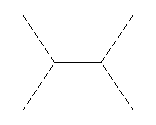
\includegraphics{Chapters/Images/nontrivM4.pdf}};
                \node at (1.2,0.7) {$x_{3}$};
                \node at (1.2,-0.7) {$x_{4}$};
                \node at (-1.2,0.7) {$x_{1}$};
                \node at (-1.2,-0.7) {$x_{2}$};
                \node[above] at (0,0) {$l$};
            \end{tikzpicture}
            \caption{Type (A)}
        \end{subfigure}
         \begin{subfigure}[b]{0.22\textwidth}
            \begin{tikzpicture}
                \node[inner sep = 0pt] at (0,0) {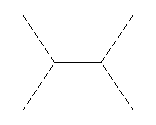
\includegraphics{Chapters/Images/nontrivM4.pdf}};
                \node at (1.2,0.7) {$x_{2}$};
                \node at (1.2,-0.7) {$x_{4}$};
                \node at (-1.2,0.7) {$x_{1}$};
                \node at (-1.2,-0.7) {$x_{3}$};
                \node[above] at (0,0) {$l$};
            \end{tikzpicture}
            \caption{Type (B)}
        \end{subfigure}       
        \begin{subfigure}[b]{0.22\textwidth}
            \begin{tikzpicture}
                \node[inner sep = 0pt] at (0,0) {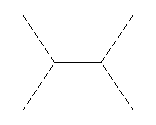
\includegraphics{Chapters/Images/nontrivM4.pdf}};
                \node at (1.2,0.7) {$x_{2}$};
                \node at (1.2,-0.7) {$x_{3}$};
                \node at (-1.2,0.7) {$x_{1}$};
                \node at (-1.2,-0.7) {$x_{4}$};
                \node[above] at (0,0) {$l$};
            \end{tikzpicture}
            \caption{Type (C)}
        \end{subfigure}
        \begin{subfigure}[b]{0.22\textwidth}
            \begin{tikzpicture}
                \node[inner sep = 0pt] at (0,0) {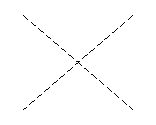
\includegraphics{Chapters/Images/trivM4.pdf}};
                \node at (1.2,0.7) {$x_{2}$};
                \node at (1.2,-0.7) {$x_{3}$};
                \node at (-1.2,0.7) {$x_{1}$};
                \node at (-1.2,-0.7) {$x_{4}$};
            \end{tikzpicture}
            \caption{Type (D)}
        \end{subfigure}
    \end{figure}
    \par These combinatorial types play an important role for the rest of this chapter, and thus we will refer to them with the captions given below each figure.
    \par The combinatorial types (A) to (C) have codimension $0$, and hence correspond to stratum of $M_{4}$ isomorphic to $\mathbb{R}_{>0}$, parametrised by the edge length $l$.
    And the combinatorial type (D) with codimension $1$ corresponds to a single point in $M_{4}$. Thus, we have the following picture for $M_{4}$, with each unbounded edge corresponding to one of the types (A), (B), or (C).
    \begin{center}
       \begin{tikzpicture}
           \draw (0,0) -- (0,2) node [left]{\emph{(A)}};
           \draw (0,0) -- (2,-1)node [above]{\emph{(B)}};
           \draw (0,0) -- (-2,-1)node [above]{\emph{(C)}};
           \node at (0,0.2) [right]{\emph{(D)}};
       \end{tikzpicture} 
    \end{center}
\end{example}


\subsection{Multilplicites and Evaluation Maps}

\begin{definition}[Morphism between polyhedra]
   For two polyhedra $X$ and $Y$, a map $f:X \to Y$ is called a polyhedral morphism if for each cell $X_{i}\subset X$, $f(X_{i})$ is contained in only one cell of $Y$, and $f|_{X_{i}}$ is a linear map. 
\end{definition}

\begin{definition}[Multiplicity of polyhedral morphisms]
    Let $X$ and $Y$ be polyhdera of same pure dimension, with $f:X\to Y$ a morphism. 
    For $Q\in X$ such that both $Q$ and $f(Q)$ are in general position, around $Q$, $f$ looks like a map between vector spaces of same dimension.
    We then define the absolute value of the determinant of this linear map as the multiplicity of $f$ at $Q$, $\text{mult}_{f}(Q)$.
    It's easy to see that this multiplicity is the same for all elements of the cell which contains $Q$, so we also refer to $\emph{mult}_{f}(Q)$ as the multiplicity of the cell.
\end{definition}

\begin{definition}[Degree of a Polyhedral Morphism]
    Let $X$ and $Y$ be polyhdera of same pure dimension, with $f:X\to Y$ a morphism. 
    We say a point $Q \in Y$ is said to be in $f$-general position if $Q$ is in general position in $Y$ and all elements of $f^{-1}(Q)$ are in general posisition in $X$.
    Then the degree of $f$ at $Q$ is defined as:
    \[
        \emph{deg}_{f}(Q):= \sum_{P \in f^{-1}(Q)}\emph{mult}_{f}(P).
    \]
    In the following remark we explain why this sum is well defined.
\end{definition}

\begin{remark}
    Firstly, note that the polyhedra $X$ and $Y$ are finite dimensional, hence they both have a finite number of cells. 
    So a finite number of cells contain the points of $f^{-1}(Q)$ (for $Q\in Y$).
    Via linearity of $f$ on each cell (of $X$) it follows that if a cell contains multiple elements of $f^{-1}(Q)$ then the determinant of the linear map is zero on that cell. 
    Hence the multiplicity of $f$ on cells containing multiple points of $f^{-1}(Q)$ is $0$.
    This leaves us with a finite number of cells, on which the map $f$ is injective, hence has non-zero multiplicity. 
    Implying that the above sum is well-defined.
\end{remark}

Evaluation maps for tropical curves are defined in the same manner as for rational plane curves.
\begin{definition}[Evaluation Maps]
    For each marked point $x_{i}$ on a $n$-pointed plane tropical curve, $(\Gamma,x_{1},\dots,x_{n},h)$ we define the evaluation map $\emph{ev}_{i}:M_{\Delta, n} \to \mathbb{R}^{2}$ as:
    \[
        (\Gamma,x_{1},\dots,x_{n},h) \to h(x_{i}).
    \]
    We denote with $\emph{ev}_{i}^{1}$ and $\emph{ev}_{i}^{2}$ the composition of the evaluation map with the projection onto the first and second coordinates respectively.
    \par The total evaluation map is defined as:
    \[
        \emph{ev} := \emph{ev}_{1} \times \dots \times \emph{ev}_{n}:M_{\Delta, n} \to \mathbb{R}^{2n}: M_{\Delta, n} \to (h(x_{1}),\dots,h(x_{n})).
    \]
\end{definition}

\begin{remark}[The Evaluation map is a morphism of polyhedra]
    
\end{remark}

\begin{remark}[Degree of total evaluation counts number of curves]
    From lemma \ref{graphLem}, when $n = |\Delta|-1$, both $M_{\Delta, n}$ and $\mathbb{R}^{2}$ have the same dimension. We then define the following number,
    \begin{align*}
        N^{\text{trop}}_{\Delta}(P) := \text{deg}_{\text{ev}}(P),
    \end{align*}
    for $P \in \mathbb{R}^{2n}$ in $\text{ev}$-general position.
    \par This number counts the number of curves $C$ of degree $\Delta$ passing through the points $P$, where each curve is given multiplicity $\text{mult}_{\text{ev}}(C)$.
\end{remark}

\begin{definition}[Rigid plane tropical curves]
    Let $C = (\Gamma, x_{1},\dots, x_{n}, h) \in M_{\Delta, n}$ be a $3$-valent plane tropical curve. 
    A subgraph $S \subset \Gamma$ is called a string if doesn't intesect with $\overline{\{x_{i}\}}$ for all $1 \leq i \leq n$.
    It's easy to see that if $C$ has a string, then the entire combinatorial type too has a string.
    Hence, we call a combinatorial type $\alpha$ rigid, if for any member curve $C$ the underlying graph $\Gamma$ has no strings.
\end{definition}

\begin{definition}[Multiplicity of a Plane tropical curve]
    Again, consided a $3$-valent plane tropical curve $C$.
    The multiplicity at a vertex $w$ of $C$ is defined as $|\emph{det}(v_{1},v_{2})|$, where $v_{1}$ and $v_{2}$ are directions of any two distinct incident flags at $v$.
    This is independent of the choice of flags due to the balancing condition, $\sum_{i}v_{i} = 0$.
    The product all all vertex multiplicities of the curve $C$ is called the multiplicity of the curve $C$, denoted $\emph{mult}(C)$.
\end{definition}
\subsection{Forgetful Maps}

Remember that forgetting marks (and the map $\mu$) for rational plane curves induced forgetful maps $\overline{\mathcal{M}}_{0,n}(\mathbb{P}^{r},d) \to \overline{\mathcal{M}}_{0,m}(\mathbb{P}^{r},d)$ and $\overline{\mathcal{M}}_{0,n}(\mathbb{P}^{r},d) \to \overline{\mathcal{M}}_{0,m}$ for $m<n$.
We now look at how one can forget marks (and the map $h$) in the context of plane tropical curves to obtain maps on the respective moduli spaces.

\begin{definition}[Forgetting the map and some points]
    Let $n\geq m$, and $C = (\Gamma, x_{1},\dots, x_{n},h) \in M_{\Delta,n}$.
    \par Let $C(m)$ be the minimal connected subgraph of $\Gamma$ which contains the undbounded edges $x_{1}, \dots, x_{m}$.
    It's clear that $C(m)$ can't contain vertices of valence $1$.
    And at vertices of valence $2$, we ``straighten" the graph - that is, replace the two neighnouring edges of lengths $l_{1},\,l_{2}$ with one edge of length $l_{1} + l_{2}$.
    The resulting graph clearly lies in $\mathcal{M}_{m}$, and we denote it by $\emph{ft}_{m}(C)$.
\end{definition}

\begin{remark}
    The ``straightening" process described in the aboce definition is the tropical analougue of \textit{stabilisation}. 
    We stablisied twigs with less that $3$ marks by contracting them to a point; here we \textit{stabilised} vertices of valence less than $3$ by straightening the graph at that point. 
\end{remark}

\begin{remark}[Forgetful maps are morphism of polyhedra]
    It's obvious that forgetful maps are morphisms of polyhedra, since we are wither forgetting coordinates (projections), or straightening (adding two coordinates), which are both linear maps. 
\end{remark}

\begin{definition}[The total map]
    Fix $d\geq 2$, $n =3d$, we define the total map:
    \begin{align*}
        \pi:= \emph{ev}^{1}_{1} \times\emph{ev}^{2}_{2} \times\emph{ev}_{3} \times \dots \emph{ev}_{n} \times \emph{ft}_{4}: M_{\Delta, n} \to \mathbb{R}^{2n-2} \times M_{4}.
    \end{align*}
\end{definition}
This map will help us consider intersection of arbritary tropical curves with, with lines $L_{1}$, $L_{2}$, and points $Q_{3}, \dots, Q_{n}$ in general position (like in the case of rational plane curves). 
This map also encodes the data of the inverse image of boundary divisors of $\mathcal{M}_{4}$ (which we used to deduce Kontsevich's formula for rational plane curves).

\begin{proposition}
    The degrees $\text{deg}_{\pi}(P)$, for $P$ in $\pi$-general position, is independent of $P$.
\end{proposition}
\begin{proof}[Sketch of proof]
    Since $\pi$ is a product of polyhedral morphisms, it follows that $\pi$ is also a morphism of polyhedra.
    As a consequence $\pi$ locally (on a cell) is an invertible linear map - hence a local isomorphism. 
    Therefore, $\text{deg}_{\pi}(P)$ is locally constant.
    \par We now need to check that the value $\text{deg}_{\pi}$ attains the same value on each maximal dimensional cell. 
    Since the polyhedral complex of the image is finite dimensional, it has a finite number of cells, and hence the set of points in $\pi$-general position are the complement of a codimension $1$ polyhedral complex. 
    That is the top dimensional cells in the image are separated by codimension $1$ walls, and we need to check if passing across any such wall conserves the degree of $\pi$.
    \par Since this wall is of codimension $1$ it follows from the definition that every element of the wall corresponds to a curve with just a single $4$-valent vertex (with the other vertices having valence $3$). 
    Consider an aribritary such wall in the image, and suppose that the combinatorial type of elements in the wall is $\alpha$, then there exist three possible combinatorial types, $\alpha_{1},\, \alpha_{2},\,\alpha_{3}$, such that $\alpha$ lies on their boundary.
    This can be seen in the following figure, illustrating the neighbourhood of the curve around the $4$-valent vertex, denoted $\alpha$, in the moduli space:
    \begin{figure}[h]
        \centering
        \begin{tikzpicture}
            %figure 1
            \node[inner sep = 0pt] at (0,0) {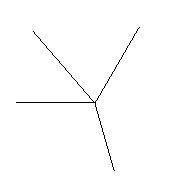
\includegraphics{Chapters/Images/degpropimg1.pdf}}; 
            \node[above] at (-0.7,0.8) {$E_{1}$};
            \node[right] at (0.5,0.7) {$E_{2}$};
            \node[right] at (0.2, -1) {$E_{3}$};
            \node[below] at (-1, -0.2) {$E_{4}$};
            \node[right] at (0,-0.2) {$V$};
            %figure 2
            \node[inner sep = 0pt] at (4,0) {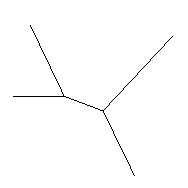
\includegraphics{Chapters/Images/degpropimg2}}; 
            \node[above] at (3.3,0.8) {$E_{1}$};
            \node at (4.5,0.7) {$E_{2}$};
            \node[left] at (4.5, -1) {$E_{3}$};
            \node[below] at (2.7, 0) {$E_{4}$};
            \node[below] at (3.5,-0.1) {$V$};
            %figure 3
            \node[inner sep = 0pt] at (7.5,0) {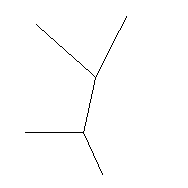
\includegraphics{Chapters/Images/degpropimg3}};
            \node[above] at (7,0.8) {$E_{1}$};
            \node[right] at (8,1.2) {$E_{2}$};
            \node[below] at (7.6, -1.3) {$E_{3}$};
            \node[above] at (6.4, -0.7) {$E_{4}$};
            \node[right] at (7.5,0.3) {$V$};
            %figure 4
            \node[inner sep = 0pt] at (10.5,0) {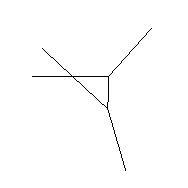
\includegraphics{Chapters/Images/degpropimg4}};
            \node[above] at (9.6,0.65) {$E_{1}$};
            \node[below] at (11.59,1.1) {$E_{2}$};
            \node[below] at (10.8, -1) {$E_{3}$};
            \node at (9.4, 0) {$E_{4}$};
            \node[right] at (10.7,0.2) {$V$};
            %others
            \draw[-Stealth, thick] (1,0) -- (2,0);
            \node at (0,-2.3){$\alpha$};
            \node at (4,-2.3){$\alpha_{1}$};
            \node at (7.5,-2.3){$\alpha_{2}$};
            \node at (10.5,-2.3){$\alpha_{3}$};
        \end{tikzpicture}
    \end{figure}

    \par Let $C$ be a reprsentative curve for the combinatorial type $\alpha$.
    We assume that all four neighbouring edges of $V$ - $E_{1}$, $E_{2}$, $E_{3}$, $E_{4}$ - are bounded (since the proof for the cases where either of them are unbounded is almost exactly the same). 
    \par Let $A$ denote the matrix for the map $\pi|_{\alpha}$ and $A_{i}$ the matrices for $\pi|_{\alpha_{i}}$.
    We need to show that $\text{det}A_{1} = \text{det}A_{3} =\text{det}A_{3}$.
    To do this we look at the following component of the matrix $A_{1}$:
    \[
        \begin{bmatrix}
            \cdots & w & l_{1} & l_{2} & l_{3} & l_{4} & l^{\alpha_{1}}\\
            \text{marked points through $E_{1}$} & I_{2} & v_{1} & 0 & 0 & 0 & 0\\
            \text{marked points through $E_{2}$} & I_{2} & 0 & v_{2} & 0 & 0 & v_{2} + v_{3}\\
            \text{marked points through $E_{3}$} & I_{2} & 0 & 0 & v_{3} & 0 & v_{2} + v_{3}\\
            \text{marked points through $E_{4}$} & I_{2} & 0 & 0 & 0 & v_{4} & 0\\
            \text{coordinate of }M_{4} & 0 & * & * & * & * & **
        \end{bmatrix},
    \]
    here, $w$ is the coordinate of the root vertex, and $l_{i}$ and $v_{i}$ the lengths and directions of the edges $E_{i}$. Further, in the last column, $l_{\alpha_{1}}$ is the length of the "new" edge in the combinatorial type $\alpha_{1}$.
    It's easy to see that the matrices $A_{i}$ for $i =2,\,3$ will differ from the above matrix only in the last column - with length of the new bounded edge and direction vectors appropriately changed.
    And the last row just corresponds to the $M_{4}$ coordinate, with $*$ and $**$'s either being $0$ or $1$.
    \par We calculate the determinant on a case by case basis - with each case corresponding to the number of $E_{i}$'s preserved under the forgetful map to $M_{4}$. 
    Here we only look at the case all $4$ of the edges are preserved under the forgetful map and leave the reader to refer to \cite{GATHMANNwdvv} for the other cases.
    \par Suppose $\text{ft}_{4}(C)$ is a curve of type (D) - then the other three combinatorial types $\alpha_{1},\, \alpha_{2},\,\alpha_{3}$ are mapped to curves of types (A), (B), and (C) under the forgetful map.
    Hence, the length parameter of the added edge in curves of types (A), (B), and (C) comes just from the last column of the matrices $A_{i}$.
    That is, in $A_{1}$ (and $A_{2}$, $A_{3}$) $* = 0$, and $** = 1$.
    It follows that the determinant of all $A_{i}$'s depends on all but the last columns othe component of the matrix we considered above, implying:
    \[
        \text{det}A_{1} = \text{det}A_{2} =\text{det}A_{3}.
    \]
\end{proof}



\section{Kontsevich's Formula}

When we studied the moduli spaces of rational curves reducible curves played an important role in constructing the moduli space, and consequently in deriving Kontsevich's curve counting formula.
We will now introduce a similar notion of \textit{reducibility} for plane tropical curves, which will motivate the next lemma. 

\par Let $(\Gamma, x_{1}, \dots,x_{n}, h)$ be a degree $d$ plane tropical curve such that there exists a bounded edge $e \in \Gamma_{0}^{1}$ which is mapped to a single point under $h$.
Further, assume that there exist atleast one bounded edge on either side of $e$.
This allows us to split the graph, $\Gamma$ into two, $\Gamma_{1}$ and $\Gamma_{2}$.
Let $v_{1}$ and $v_{2}$ denote the two verticed adjacent to $e$ in the graph $\Gamma$.
Let $U_{i}$ denote the connected compnent of the graph $\Gamma \setminus \{e\}$ containing the vertex $v_{i}$ (for $i = 1,\,2$).
Each $U_{i}$ in its own right a graph. 
Construct $\Gamma_{i}$ by adding an \textit{end} $R_{i}$ to each component $U_{i}$ such that $R_{i}$ is adjacent to the vertex $v_{i}$, that is, 
\begin{align*}
    \Gamma_{i} = U_{i} \cup \{R_{i}\}~~~\text{for }i=1,\,2.
\end{align*}
Clearly these graphs are also abstracted tropical curves. 
Now identify $m_{i}$ marked points on each $\Gamma_{i}$ - the marked points $x_{1}, \dots, x_{n}$ which lie on each component $U_{i}$ along with the ends $R_{i}$.
Since $R_{i}$ are marked points on each $\Gamma_{i}$ they will be mapped to a point under the map $h$ and hence we have maps $h_{i}$ from each component abstract tropical curve into $\mathbb{R}^{2}$.
This finally gives us two pointed plane tropical curves, $C_{1}$ and $C_{2}$, which we obtained from splitting the original curve at a contracted bounded edge.
Further, via the balancing condition it's easy to see that if $C_{1}$ and $C_{2}$ have degrees $d_{1}$ and $d_{2}$, respectively, then $d_{1} + d_{2}=d$.

\begin{remark}
    Plane tropical curves $C$ which satisfy the assumptions used to construct the two component curves above are said to be \textit{reducible}.
\end{remark}

\begin{lemma}
    \label{redCond}
    Let $d \geq 2$, $n=3d$, and $P \in \mathbb{R}^{2n-2}\times M_{4}$ be in $\pi$-general position such that the $M_{4}$ coordinate of $P$ is of type (A), (B), or (C), with large length coordinate, then:
    \begin{itemize}
        \item every plane tropical curve $C \in \pi^{-1}(P)$ with $\text{mult}_{\pi}(C) \neq 0$ has a contracted bounded edge.
    \end{itemize}
\end{lemma}
\begin{proof}
    Refer to Proposition 5.1 inProposition 5.1 in  \cite{GATHMANNwdvv} for the proof.
\end{proof}

The next lemma formalies a counting argument we repeatedly used in the proof of Kontsevich's formula to eliminate boundary divisors with zero contribution.
Making use of the remark \ref{why3d1points} we were repeatedly able impose bounds on the degree of the twigs of the boundary divisors.
The following lemma impose a similar restriction on the number of marked points on each component of a reducible plane tropical curve $C$.

\begin{lemma}
    \label{reduCntLem}
   Let $P = (a,b, p_{3}, \dots, p_{n}, z) \in \mathbb{R}^{2n-2} \times M_{4}$ be a point in $\pi$-general poisition such that the $M_{4}$ coordinate corresponds to a type (A) curve with large lentgth coordinate. 
   If $C \in \pi^{-1}(P)$, then either of the following is true:
   \begin{enumerate}
       \item $x_{1}$ and $x_{2}$ are adjacent to the same vertex. This vertex maps to $(a,b)$ under $h$.
       \item $C$ is reducible and decomposes uniquely into components $C_{1}$ and $C_{2}$ of degrees $d_{1}$ and $d_{2}$. 
           The marks $x_{1}$ and $x_{2}$ lie on the same component $C_{1}$, and $x_{3}$ and $x_{4}$ lie on the same component $C_{2}$.
           Further, $3d_{1}-1$ of the remaining marks lie on $C_{1}$.
   \end{enumerate}
\end{lemma}
\begin{proof}
    From lemma \ref{redCond}, if $C \in \pi^{-1}(P)$ with $\text{mult}_{\pi}(C) \neq 0$, then $C$ has atleast one bounded contracted edge.
    It's also true that there can exists only one such edge, else if there existed $2$ bounded contracted edges, we would have $2n-3$ coordinates (in $M_{d,n}$) determining $2n-2$ coordinates in the image, implying $\text{mult}_{\pi}(C) = 0$, which is a contradiction.
    Call the unique contracted bounded edge $E$.
    We claim that $E$ lies in the image of the forgetful map $\text{ft}_{4}(C)$.
    Because if this wasn't true, the $M_{4}$ coordinate of $P$ wouldn't have a large length parameter - contradicting the hypothesis.
    \par If $x_{1}$ and $x_{2}$ are incident at $E$, the curve $C$ is not reducible (by definition).
    Therefore $x_{1}$ and $x_{2}$ are mapped to the same point $(a,b) \in \mathbb{R}^{2}$.
    \par If $x_{1}$ and $x_{2}$ are not incident at $E$, then there exists a bounded edge on either side of $E$, making $C$ reducible.
    Say $C$ splits into component $C_{1}$ and $C_{2}$, and $x_{1},\,x_{2}$ lie on the component $C_{1}$.
    Then, $x_{1}$ and $x_{2}$ can't be incident on the same vertex in $C_{1}$ - since then, $C_{1}$ would have a bounded contracted edge, implying $C$ has a bounded contracted edge other than $E$, which we proved was not possible.
    \par We now need to count the number of marks on each component $C_{1}$ and $C_{2}$.
    Let $n_{1}$ and $n_{2}$ denote the number of remaining marks from $x_{5}, \dots, x_{n}$ which lie on $C_{1}$ and $C_{2}$, respectively.
    If $n_{1} = 3d_{1} - 1$, then since $n = 3d_{1} + 3d_{2} = n_{1}+n_{2}+4$, we also get the condition $n_{2} = 3d_{2} - 3$.
    Now suppose $n_{1} \geq 3d_{1}$:
    \begin{itemize}
        \item The image of $C_{1}$ under $h$ has $2n_{1}+6\geq 3d_{1} + n_{1} + 5 $ coordinates - $2$ from the root vertex, and $2$ coordinates for every marked point.
        \item But since the underlying graph of $C_{1}$ has $3d_{1}+ n_{1}+ 2$ unbounded ends, there exist $3d_{1}+ n_{1} -1 $ number of bounded edges.
        \item Hence, we are trying to determine more than $3d_{1} + n_{1} + 5$ entries from $3d_{1}+ n_{1} +1$ coordinates, implying $\text{mult}_{\pi}(C_{1}) = 0$, which is a contradiction.
    \end{itemize}
    Therefore $n_{1} \leq 3d_{1}-1$.
    Similarly, we can show that $n_{2} \leq 3d_{2}-3$.
    But since $n_{1}+n_{2} = (3d_{1}-1) + (3d_{2}-3)$, the previous inequalities become equalities, implying $n_{1} = 3d_{1}-1$, thus finishing the proof.
\end{proof}

This result motivates us to ask if we can count $\pi$-multiplicities of the curve $C$ by bounting $\pi$-multiplicities of its components?
In the following remark we show that this is indeed possible.

\begin{remark}
    \label{convReduCnt}
    To be able to count $\pi$-multiplicites of $C$ with its component curves we need to see if this decomposition is unique?
    That is, if $C_{1}$ and $C_{2}$ are plane tropical curves of degrees $d_{1}$ and $d_{2}$, with $d_{1}+d_{2}=d$, such that there exists a point $ P = (a,b, p_{3}, \dots, p_{n}, z) \in \mathbb{R}^{2n-2} \times M_{4}$ 
    with $z$ having large length coordinate, $C_{1}$ passing through lines $L_{1} = \{x = a\}$, $L_{2} = \{y = b\}$ and $3d_{1}-1$  marks form $p_{5},\dots, p_{n}$, and $C_{2}$ passes through $p_{3}$, $p_{4}$ and the remaining $3d_{2}-3$ marks - does there exist a unique curve $C$ whose components are $C_{1}$ and $C_{2}$?
    \par It indeed does! Check remark 5.4 of \cite{GATHMANNwdvv} for the details.
\end{remark}


\begin{proposition}
    \label{multCntProp}
    Consider a point $P$ in $\mathbb{R}^{2n-2}\times M_{4}$, and let $C \in \pi^{-1}(P)$, then either of the following is true:
    \begin{enumerate}
        \item if $C$ is of type $1.$ from lemma \ref{reduCntLem}, if we denote with $C'$ the curve obrained by forgetiing the mark $x_{1}$ and $\text{ev}$ denotes the evaluation map for the remaining marks:
            \[
                \text{mult}_{\text{ev}}(C') = \text{mult}_{\pi}(C);
            \]
        \item if $C$ is of type $2.$ from lemma \ref{reduCntLem} then:
            \[
                \text{mult}_{\pi}(C) = \text{mult}_{\text{ev}}(C_{1}) \cdot \text{mult}_{\text{ev}}(C_{2}) \cdot (C_{1}\cdot C_{2})_{R_{1} = R_{2}} \cdot (C\cdot L_{1})_{x_{1}} \cdot (C\cdot L_{2})_{x_{2}},
            \]
    \end{enumerate}
    where $R_{1}=R_{2}$ corresponds to the point of intersection of the curves $C_{1}$ and $C_{2}$ obtained by splitting $C$ along the contracted bounded edge, and $(C_{j}\cdot L_{i})_{x_{i}}$ denotes the $i^{\text{th}}$ coordinated of the direction vector of $C_{j}$ at $x_{i}$.
\end{proposition}
\begin{proof}
    Refer to \cite{GATHMANNwdvv} for the proof.
\end{proof}

We now (finally) derive Kontsevich's formula for plane tropical curves.
\begin{theorem}
    The number $N_{d}^{\text{trop}}$, for $d>1$, satisfies the following reccurence relation,
    \begin{align*}
        N^{\text{trop}}_{d} = \sum_{\substack{d_{1}+d_{2}=d;\\ d_{1},\,d_{2}\geq1}}
        \left( d_{1}^{2}d_{2}^{2} \binom{3d-4}{3d_{1}-2} - d_{1}^{3}d_{2}\binom{3d-4}{3d_{1}-1} \right) N^{\text{trop}}_{d_{1}}N^{\text{trop}}_{d_{2}}.
    \end{align*}
\end{theorem}
\begin{proof}
    As hinted at the start of this section, we compute the degree of $\pi$ at two different points in $\mathbb{R}^{2n-2}\times M_{4}$, and equate them to arrive at the formula.
    Consider points $\mathcal{P} = (a,b,p_{3}, \dots, p_{n},z)$ and $\mathcal{P}' = (a',b',p_{3}', \dots, p_{n}',z')$ in $\mathbb{R}^{2n-2}\times M_{4}$ in $\pi$-general position. 
    We choose these points such that $z$ and $z'$ correspond to curves of type (A), and type (B) respectively.
    \par \textit{\textbf{I.} Computing the degree at $\mathcal{P}$}, $\text{deg}_{\pi}(\mathcal{P})$.
    \par As discussed in lemma \ref{reduCntLem}, curves in $\pi^{-1}(P)$ can be of two types - we call them type $1$ and type $2$ curves.
    The multiplicity of $\pi$ at type $1$ curves, counts number of degree $d$ curves passeing though the $3d-2$ marks, $p_{3}, \dots, p_{n}$, and the point $(a,b) \in \mathbb{R}^{2}$.
    That is the $\pi$-multiplicity at type $1$ curves counts the number of degree $d$ curves passing through $3d-1$ points (with $\text{ev}$-multiplicity), which by definition is the number $N^{\text{trop}}_{d}$.
    \par Now consider curves of type 2.
    From remark \ref{convReduCnt} we can compute the $\pi$-multiplicity of $C$ by computing $\pi$ multiplicities of the components $C_{1}$ and $C_{2}$ appropriately (following proposition \ref{multCntProp}).
    We will also need to account for the number of such decompositions possible to compute the multiplicity; again from remark \ref{convReduCnt}, the data of the component curves $(C_{1},C_{2},x_{1},\dots,x_{n},P,Q)$ are characterised by the following properties:
    \begin{enumerate}
        \item $\text{deg}C_{1} = d_{1}$ and $\text{deg}C_{2} = d_{2}$, such that $d_{1}+d_{2}=d$.
        \item $x_{1}$ and $x_{2}$ are marked points on $C_{1}$ that map to $L_{1}$ and $L_{2}$.
        \item $x_{3}$ and $x_{4}$ are marked points on $C_{1}$ that map to $p_{3}$ and $p_{4}$.
        \item $x_{5},\dots,x_{n}$ map to $p_{5},\dots,p_{n}$, with $3d_{1}-1$ of them lying on $C_{1}$.
        \item $P \in C_{1}$ and $Q \in C_{2}$ are mapped to the same point in $\mathbb{R}^{2}$.
    \end{enumerate}
    From $4.$ above, there are $\binom{3d-4}{3d_{1}-1}$ possible ways of distributing the marks.
    For each such distribution of marks, from the previous proposition, the multiplicity is given by the expression:
    \begin{align*}
        \text{mult}_{\text{ev}}(C_{1}) \cdot \text{mult}_{\text{ev}}(C_{2}) \cdot (C_{1}\cdot C_{2})_{P=Q} \cdot (C\cdot L_{1})_{x_{1}} \cdot (C\cdot L_{2})_{x_{2}}.
    \end{align*}
    Using B\'{e}zout's theorem for tropical curves we can compute each of the intersection multiplicites above.
    \begin{itemize}
        \item $\text{mult}_{\text{ev}}(C_{1}) = N^{\text{trop}}_{d_{1}}$.
        \item $\text{mult}_{\text{ev}}(C_{2}) = N^{\text{trop}}_{d_{2}}$.
        \item $(C_{1}\cdot C_{2})_{P=Q} = d_{1}d_{2}$.
        \item $(C\cdot L_{1})_{x_{1}} = d_{1}$.
        \item $(C\cdot L_{2})_{x_{2}} = d_{1}$.
    \end{itemize}
    Hence, it follows:
    \begin{align*}
        \text{deg}_{\pi}(\mathcal{P}) = N_{d}^{\text{trop}} + \sum_{\substack{d_{1}+d_{2}=d;\\ d_{1},\,d_{2}\geq1}}
        d_{1}^{3}d_{2}\binom{3d-4}{3d_{1}-1}  N^{\text{trop}}_{d_{1}}N^{\text{trop}}_{d_{2}}.
    \end{align*}
    \par \textit{\textbf{II.} Computing the degree at $\mathcal{P}'$}, $\text{deg}_{\pi}(\mathcal{P}')$.
    \par We can repeat the same steps as for part \textit{\textbf{I.}} and deduce that:
    \begin{align*}
        \text{deg}_{\pi}(\mathcal{P}') =  \sum_{\substack{d_{1}+d_{2}=d;\\ d_{1},\,d_{2}\geq1}}
        d_{1}^{2}d_{2}^{2}\binom{3d-4}{3d_{1}-2}  N^{\text{trop}}_{d_{1}}N^{\text{trop}}_{d_{2}}.
    \end{align*}

    Since degree of $\pi$ is independent of points $\mathcal{P}$ in general position, Kontsevich's equation follows.
\end{proof}
